\documentclass[xcolor=x11names,compress,aspectratio=169]{beamer}
%\documentclass[xcolor=x11names,compress,aspectratio=43]{beamer}

%% General document %%%%%%%%%%%%%%%%%%%%%%%%%%%%%%%%%%
\usepackage{graphicx}
\usepackage{tikz}
\usepackage{amsmath}
\usepackage{amssymb}
\usepackage[utf8]{inputenc}
\usepackage{textpos}
\usepackage{booktabs}
\usepackage{listings}
\usepackage{auto-pst-pdf}

\usetikzlibrary{decorations.fractals, calc}
%%%%%%%%%%%%%%%%%%%%%%%%%%%%%%%%%%%%%%%%%%%%%%%%%%%%%%

%% Beamer Layout %%%%%%%%%%%%%%%%%%%%%%%%%%%%%%%%%%
\useoutertheme[subsection=false,shadow]{miniframes}
\useinnertheme{default}
%\usefonttheme{serif}
\usepackage{palatino}
\setbeamerfont{title like}{shape=\scshape}
\setbeamerfont{frametitle}{shape=\scshape}
\beamertemplatenavigationsymbolsempty


% Uncomment this line, if you want frame numbers on your slides
% (I disabled them since I had the progress bar at the header)
%\setbeamertemplate{footline}[frame number]

\definecolor{fmiBlue}{RGB}{11,128,145} % FSU Faculty blue
\definecolor{evbc}{RGB}{50,167,132} % EVBC Green
\definecolor{bgGray}{RGB}{230,230,230} % some gray if needed


\setbeamercolor*{upper separation line head}{bg=Snow4} %Snow4 comes from the x11names option of xcolor
%\setbeamercolor*{lower separation line head}{bg=evbc}  % obsolete - there is now a cool progress bar 
\setbeamercolor*{normal text}{fg=black,bg=white} 
\setbeamercolor*{alerted text}{fg=red} 
\setbeamercolor*{example text}{fg=black} 
\setbeamercolor*{structure}{fg=black} 
 
\setbeamercolor*{palette tertiary}{fg=black,bg=black!10} 
\setbeamercolor*{palette quaternary}{fg=black,bg=black!10} 

%%%%%%%%%%%%%%%%%%%%%%%%%%%%%%%%%%%%%%%%%%%%
% IMPORTANT
% Kevin:
% Currently the FMI blue (the light uni blue) is here.
% If you want for example the evbc green, you'd have to
% change the colors here. I will put this in a nice function
% at some point.
\setbeamercolor{title}{fg=evbc}
\setbeamercolor{structure}{fg=evbc}
\setbeamercolor{frametitle}{fg=evbc}
\setbeamercolor{block title}{fg=evbc, bg=bgGray}
\setbeamercolor{block title example}{fg=evbc}
\setbeamercolor{enumerate item}{fg=evbc}
\setbeamercolor{itemize item}{fg=evbc}
\setbeamercolor{item projected}{bg=evbc}

\setbeamerfont{block title}{size=\small}
\setbeamerfont{block body}{size=\scriptsize}

% Use those if you want. Just some shortcuts for 
% columns. Personally, I use minipages nowadays.
\renewcommand{\(}{\begin{columns}}
\renewcommand{\)}{\end{columns}}
\newcommand{\<}[1]{\begin{column}{#1}}
\renewcommand{\>}{\end{column}}

% Kevin:
% This is used for the code examples in the document.
% If used, set the frame option to 'fragile' (!!!)
\lstset{
	language=sh, 
	numbers=left, 
	numberstyle=\tiny\color{gray}, 
	backgroundcolor=\color{bgGray}, 
	basicstyle=\scriptsize\ttfamily,
	commentstyle=\tiny\color{Green4},
	keywordstyle=\color{Blue3},
	escapeinside=@@
}

% Kevin
% Appendix page number fix. More like an ugly hack.
% I was never able to create a "nice" appendix command, however, this one here works fine.
\newcommand{\beginbackup}{
   \newcounter{framenumbervorappendix}
   \setcounter{framenumbervorappendix}{\value{framenumber}}
}
\newcommand{\backupend}{
   \addtocounter{framenumbervorappendix}{-\value{framenumber}}
   \addtocounter{framenumber}{\value{framenumbervorappendix}} 
}

%%%%%%%%%%%%%%%%%%%%%%%%%%%%%%%%%%%%%%%%%%%%%%%%%%
% Kevin: Change this, if you want.
\graphicspath{{figures/}}
%

% Kevin:
% I used this slides for subsections a long time ago, however, at some point I figured that it is nicer to have those slides
% at the beginning of each section. Use this extra slides to give a short summary of the previous talk.
\AtBeginSection[]{
  \begin{frame}
  \vfill
  \centering
  \begin{beamercolorbox}[sep=8pt,center,shadow=true,rounded=true]{title}
    \usebeamerfont{title}\insertsection\par%
  \end{beamercolorbox}
  \vfill
  \end{frame}
}


% Kevin:
% small macro, used to build the progress bar
\def\insertframeratio{%
    \pgfmathparse{\insertframenumber/\inserttotalframenumber}%
}
%%%%%%%%%%%%%%%%%%%%%%%%%%
% Kevin:
% This is the progress bar in the headline.
% Change the textcolor if needed, change the width to 2pt if wanted
\addtobeamertemplate{headline}{}{%
  \insertframeratio
  \edef\myvar{\pgfmathresult}
  %\textcolor{evbc}{\rule{\myvar \paperwidth}{1pt}}
  \textcolor{evbc}{\rule{\paperwidth}{1pt}}
}

%%%%%%%%%%%%%%%%%%%%%%%%%%%
% Kevin
% This adds the FSU Logo to the
% bottom left. Changing the logo is easy
% adding a second logo (e.g. the evbc) is tricky
\addtobeamertemplate{footline}{}{%
\begin{textblock*}{100mm}(1em,-3.5em)

\includegraphics[scale=0.4]{evbc_cmyk.pdf}
\end{textblock*} 
\begin{textblock*}{100mm}(73em,-1em) 
\insertframenumber/\inserttotalframenumber
\end{textblock*}
}

%% Kevin:
%% I used this in order to show two logos at the same time.
%% as you can see, it is quite tricky in terms of positioning 
%% and size, but a nice try-and-error session usually
%% works out.
%\addtobeamertemplate{footline}{}{%
%\begin{textblock*}{100mm}(0.5em,-5em)
%
\includegraphics[scale=0.5]{figures/evbc_cmyk.pdf}
%\end{textblock*}
%\begin{textblock*}{100mm}(11em,-3em)
%
\includegraphics[scale=0.025]{fsu_logo.jpg}
%\end{textblock*}
%}


% Kevin:
% Well, fill this out as needed
%\title{Theoretical and practical metagenomic approaches to viral discovery}
%\subtitle{}
%\author{Kevin Lamkiewicz, Manja Marz}
%\date{27.09.2018\\[1em]RNA Bioinformatics and High-Throughput Analysis\\[1em]Friedrich Schiller University Jena}
%\date{xx.xx.2018\\RNA Bioinformatics and High-Throughput Analysis\\[2em]
\includegraphics[scale=0.05]{fsu_logo.jpg}}



\title{Theoretical and practical metagenomic approaches to viral discovery}
\subtitle{Practical Session: Infernal and covariance models}
\author{Kevin Lamkiewicz, Manja Marz}
\date{25.10.2019\\[1em]European Virus Bioinformatics Center}

\begin{document}

\begin{frame}
  \maketitle
\end{frame}

\begin{frame}[c, fragile]\frametitle{Infernal}
  \texttt{http://eddylab.org/infernal}
  \begin{block}{User's Guide Quote:}
      \textbf{How to avoid reading this manual}\\
      If you’re like most people, you don’t enjoy reading documentation. You’re probably thinking: 113 pages
      of documentation, you must be joking!
  \end{block}

  \uncover<2->{
  \begin{minipage}{0.5\textwidth}
      \begin{figure}[htbp]
          \centering
          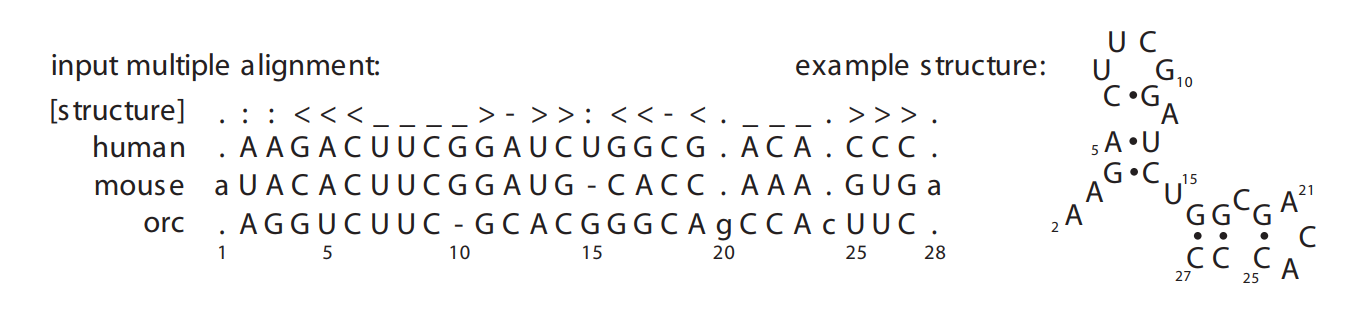
\includegraphics[width=0.95\textwidth]{figures/sequence_struc.png}          
      \end{figure}
  \end{minipage}\hfill \uncover<3->{\begin{minipage}{0.49\textwidth}
      \begin{figure}[htbp]
          \centering
          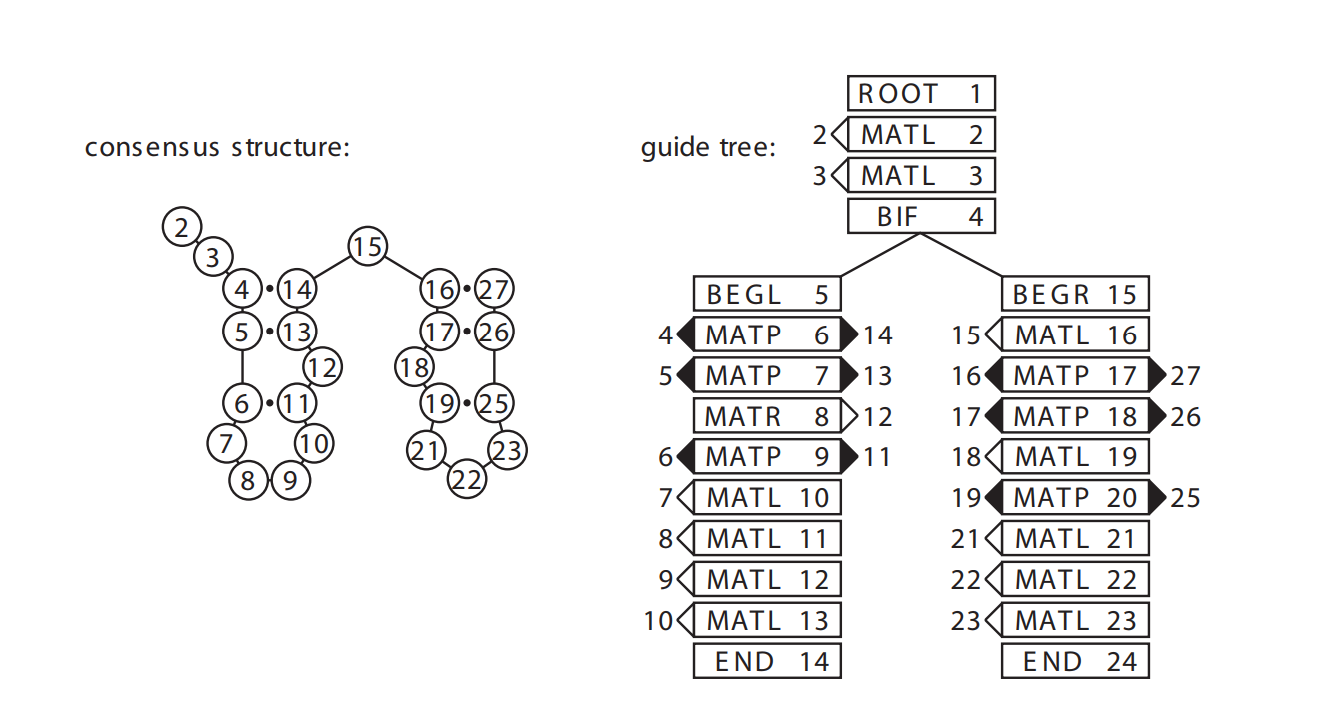
\includegraphics[width=0.95\textwidth]{figures/struc_tree.png}
      \end{figure}
  \end{minipage}
  }}

\end{frame}

\begin{frame}[c]{}
    \begin{block}{Use case}
        Given a metagenomic sample, let's assume we already assembled the reads to contigs.
        We suspect that viruses related to the Alphacoronaviruses are present in our sample, however,
        the sequence similarity is not sufficiently high for conventional methods like \texttt{blast} 
        or hidden markov-models.
    \end{block}
    \uncover<2->{
        \begin{block}{Restriction}
            Since scanning with Infernal takes quite a while, we won't use a real metagenomic sample today.
            Instead, we will download some genomes from the NCBI database - the procedure is the same for "real
            metagenomes", but faster.
        \end{block}
    }
\end{frame}



\begin{frame}[c, fragile]\frametitle{CMbuild}
    In order to build a covariance model, we need an alignment.\\
    \texttt{CMbuild} can handle \texttt{stockholm} and \texttt{CLUSTAL} format.
\begin{lstlisting}
# go to: https://www.ncbi.nlm.nih.gov/nuccore
# txid693996[Organism:exp] AND complete genome[Title]
# download them: all_complete_acov.fasta
@\pause@
# build cm from aln alignment
$> mlocarna --stockholm corona_5utr.fasta
# or clustalw corona_5utr.fasta
@\pause@
$> cmbuild corona_5utr.cvm corona_5utr.out/results/result.stk
# or cmbuild --noss corona_5utr.cvm corona_5utr.aln
\end{lstlisting}
\vspace{2em}
\uncover<4->{Which one of the two approaches is more reasonable?}
\end{frame}

\begin{frame}[c,fragile]\frametitle{CMcalibrate}
    \begin{lstlisting}
# now we calibrate our covariance model
# thus, the emission and transition probabilities are trained
# this takes quite a while
$> cmcalibrate --cpu 4 corona_5utr.cvm
    \end{lstlisting}
\vspace{2em}
\uncover<2->{
    \begin{block}{I prepared something beforehand...}
        Since \texttt{cmcalibrate} takes quite a while, even for such a small
        dataset, I already calibrated the covariance model beforehand.
        You find the CM here:\\
        \texttt{TODO}
    \end{block}
}
\end{frame}

\begin{frame}[c, fragile]\frametitle{CMsearch}
    \begin{lstlisting}
# One last step - now we search for sequences (or fragments),
# that fit to our covariance model.

# search in the fasta file for sequences matching
# the cmfile and get their positions as table

$> cmsearch --cpu 4 --tblout corona_5utr_cmsearch.csv corona_5utr.cvm \ 
        all_complete_acov.fa > cmsearch.log
    \end{lstlisting}
\end{frame}

\begin{frame}[t]\frametitle{Results}
  \begin{figure}
    \centering
    \hspace*{-2em}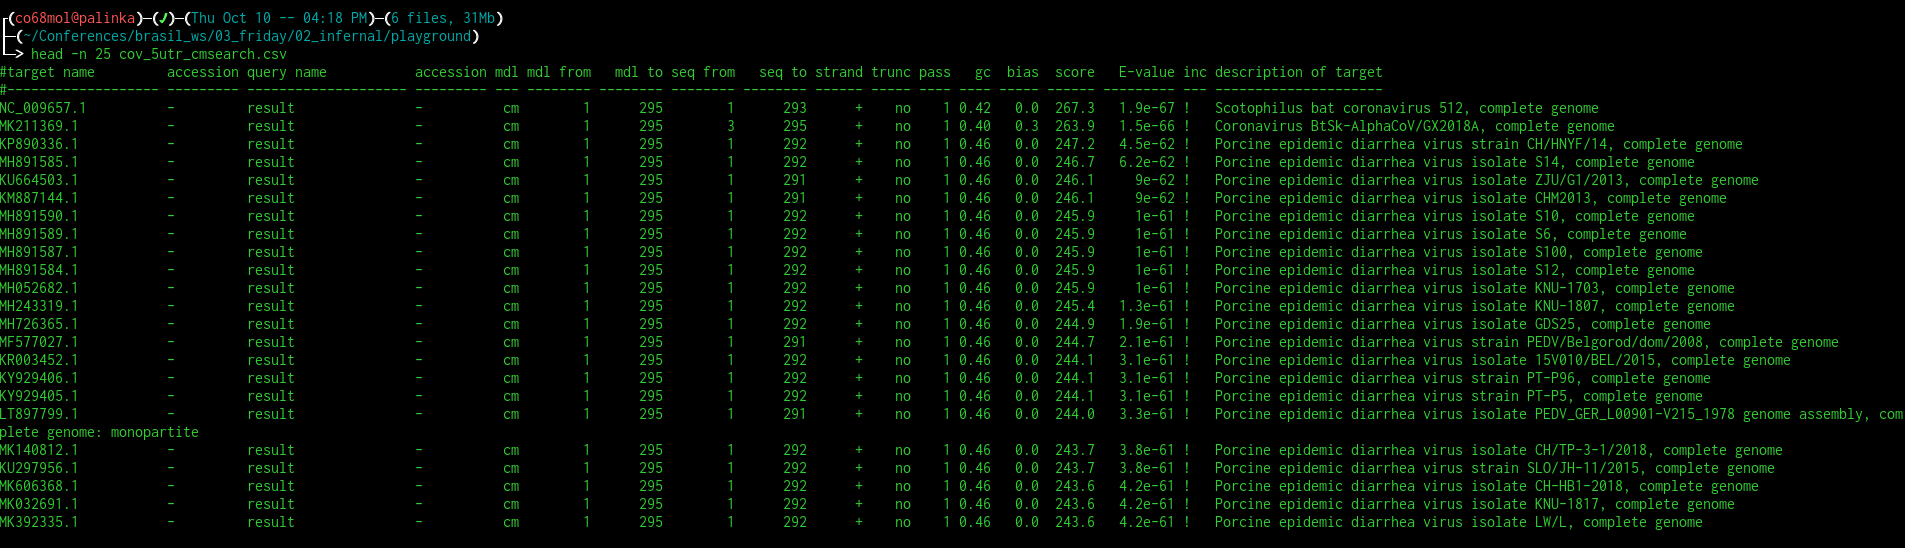
\includegraphics[width=1.1\linewidth]{cmsearch_output.png}
  \end{figure}
\end{frame}

\begin{frame}[c]\frametitle{Thanks and goodbye}
    \begin{center}
    	\includegraphics<1->[width=1\textwidth]{figures/sequence_sim.pdf} \\ \vfill
    	\includegraphics<2->[width=1\textwidth]{figures/structure_sim.pdf}
   	\end{center}
\end{frame}

% # train emission and transition probabilities
% $> cmcalibrate --cpu 2 corona_5utr.cvm
% @\pause@
% # search in the fasta file for sequences matching
% # the cmfile and get their positions as table
% $> cmsearch --cpu 2 --tblout corona_5utr_cmsearch.csv corona_5utr.cvm \ 
%         all_complete_acov.fa > cmsearch.log

% Backup Slides. Using this macro, you'd get a slide number for each
% backup slide without increasing the maximum slide numbers of the original presentation.
% However, for this, the framenumber has to be inserted - which isn't in the template by default
\beginbackup

\backupend

\end{document}